\section{Application web full-stack}
\label{chap:webapp}

L'application web expose aux utilisateurs de SOYAFF la base consolidée par le pipeline ETL (section~\ref{chap:etl}). Elle repose sur React~18 côté client et Express~4 côté serveur, avec une authentification par jetons signés et trois rôles. Le module conversationnel, bien que relayé par le même backend, est traité à part (section~\ref{chap:ia_rag}).

Les captures établissent que chaque fonctionnalité existe et fonctionne sur le système déployé ; leur valeur pour SOYAFF est mesurée au chapitre~\ref{chap:evaluation}. Le texte justifie les décisions qu'aucun écran ne montre. Le Tableau~\ref{tab:couverture_webapp} indique, exigence par exigence, ce qui tourne en production au 27~septembre~2026.

\begin{table}[htbp]
\centering
\footnotesize
\caption{Couverture des exigences applicatives par la réalisation (état au 27~septembre~2026)}
\label{tab:couverture_webapp}
\begin{tabularx}{\linewidth}{|>{\raggedright\arraybackslash}p{2.0cm}|>{\raggedright\arraybackslash}p{3.1cm}|>{\raggedright\arraybackslash}X|>{\raggedright\arraybackslash}p{1.5cm}|}
\hline
\rowcolor[HTML]{EFEFEF}
\textbf{Exigence} & \textbf{Fonctionnalité} & \textbf{Réalisation} & \textbf{État} \\ \hline

\texttt{EF-DSH-01} & Suivi de caisse en temps réel & \texttt{GET /api/stats} (lecture seule, agrégats parallèles) & \textbf{Déployé} \\ \hline
\texttt{EF-DSH-02}, \texttt{EF-DSH-04} & Visualisation de la flotte, profil véhicule & \texttt{CamionsPage.jsx} : liste, filtres, détail via \texttt{GET /api/camions} et \texttt{GET /api/camions/:id} & \textbf{Déployé} \\ \hline
\texttt{EF-DSH-03} & Classification société / particulier & Affichage typé (\texttt{type\_propriete}), bascule société~$\rightarrow$~particulier gérée à l'upsert & \textbf{Déployé} \\ \hline
\texttt{EF-SDR-01} & Saisie directe d'une opération financière & Page \texttt{SaisiePage.jsx} (\texttt{OperationForm.jsx}) $\rightarrow$ \texttt{POST /api/finances/operation} (transaction SQL atomique) & \textbf{Déployé} \\ \hline
\texttt{EF-SDR-02} & Contrôle des délais entre opérations d'un même camion & \texttt{utils/delais.js}, appliqué par l'API : frais de route bloqués sous 8~jours ; rations bloquées sous 2~jours, alerte à confirmer entre 2 et 5~jours ; forçage réservé à l'administrateur, tracé & \textbf{Déployé} \\ \hline
\texttt{EF-REP-01}, \texttt{EF-REP-02} & Récapitulatif journalier et mensuel consolidé & \texttt{GET /api/rapports/mois}, \texttt{GET /api/rapports/mensuel} & \textbf{Déployé} \\ \hline
\texttt{EF-REP-03} & Export CSV / Excel / PDF & CSV conforme Excel-FR (BOM~UTF-8, séparateur~\texttt{;}) et XLSX (\texttt{exceljs}) déployés ; PDF absent côté serveur, le bouton correspondant déclenche un \texttt{window.print()} navigateur & \textbf{Partiel} \\ \hline
\texttt{EF-REP-04} & Recherche multi-critères & Filtres période / camion / catégorie (\texttt{FinancesPage.jsx}, \texttt{RapportsPage.jsx}) & \textbf{Déployé} \\ \hline
\texttt{EF-VAL-02} & Workflow de validation numérique dématérialisé & Aucun statut de workflow en base ; insertion directe et définitive de la transaction & \textbf{Cible} \\ \hline
\texttt{EF-ADM-01} & Gestion des utilisateurs et des rôles & CRUD complet (\texttt{routes/admin.js}) : création, activation/désactivation, changement de rôle & \textbf{Déployé} \\ \hline
\texttt{EF-ADM-02} & Consultation des journaux d'audit & Onglet audit \texttt{AdminPage.jsx} $\rightarrow$ \texttt{GET /api/admin/audit}, table \texttt{audit\_logs} & \textbf{Déployé} \\ \hline
\texttt{ENF-SEC-01} & Authentification par jetons signés & JWT d'accès (8~h) + jeton de rafraîchissement (7~jours, haché SHA-256 en base) & \textbf{Déployé} \\ \hline
\texttt{ENF-SEC-02} & Hachage des mots de passe & \texttt{bcrypt}, coût~12 & \textbf{Déployé} \\ \hline
\texttt{ENF-SEC-03} & Contrôle d'accès basé sur les rôles & Contrainte \texttt{CHECK} SQL + middleware \texttt{authorize()} : \texttt{DAKAR\_AGENT}, \texttt{BAMAKO\_CHEF}, \texttt{ADMIN} & \textbf{Déployé} \\ \hline
\texttt{ENF-SEC-04} & Piste d'audit des actions sensibles & Table \texttt{audit\_logs} horodatée (connexions, refus d'accès, actions admin) & \textbf{Déployé} \\ \hline
\texttt{ENF-DISP-01} & Mode dégradé hors-ligne, cache local des saisies & Aucune trace de code (pas de \textit{service worker}, pas de file d'attente locale) & \textbf{Cible} \\ \hline
\end{tabularx}
\end{table}

Le socle de sécurité et le cœur métier (saisie, tableau de bord, reporting, administration) sont déployés et utilisés en production. Un point est partiel : l'export PDF, qui n'est qu'une impression du navigateur. Deux exigences \textit{Should} restent des cibles : le workflow de validation (\texttt{EF-VAL-02}) et le mode hors-ligne (\texttt{ENF-DISP-01}). La discussion de ces écarts est renvoyée à la section~\ref{chap:discussion}.

\subsection{Architecture applicative générale}
\label{sec:webapp_architecture}

La vue de conteneurs (Figure~\ref{fig:c4_conteneurs}) situe la pile : une \textit{single-page application} React~18 consomme une API REST Express~4 adossée à PostgreSQL. Deux choix d'organisation interne, invisibles sur les diagrammes, méritent d'être justifiés.

\textbf{Côté client, pas de routeur.} La vue affichée est portée par un simple état local dans \texttt{App.jsx}. Pour sept vues fixes, un routeur n'apportait rien. Le coût est double : aucune vue n'a d'URL propre, et la garde d'accès à l'administration est répétée au point de rendu au lieu d'être centralisée. Ce second point n'ouvre pas de faille : l'API vérifie elle-même le rôle (\S\ref{sec:webapp_rbac}), et contourner l'interface ne donnerait accès qu'à un écran vide.

\textbf{Côté serveur, le SQL dans les routes.} Les gestionnaires Express exécutent leurs requêtes directement, sans couche de service. Seule l'authentification, partagée par plusieurs routes, est isolée dans \texttt{authService.js}. Introduire une couche d'abstraction pour des routes qui n'ont qu'un appelant aurait été de la sur-ingénierie ; le découpage en couches est planifié dans le suivi du projet.

\subsection{Parcours de l'utilisateur}
\label{sec:webapp_parcours}

L'utilisateur se connecte par courriel et mot de passe (Figure~\ref{fig:web_connexion}). Le menu qu'il obtient dépend de son rôle : l'onglet \textit{Administration} n'apparaît que pour le rôle \texttt{ADMIN}. Le tableau de bord (Figure~\ref{fig:ui_dashboard}) réalise \texttt{EF-DSH-01} : solde de caisse, entrées, dépenses, flotte active, classement des camions et répartition des coûts, tous calculés côté serveur. Le bouton \textit{Assistant IA} ouvre le module décrit à la section~\ref{chap:ia_rag}.

\begin{figure}[H]
    \centering
    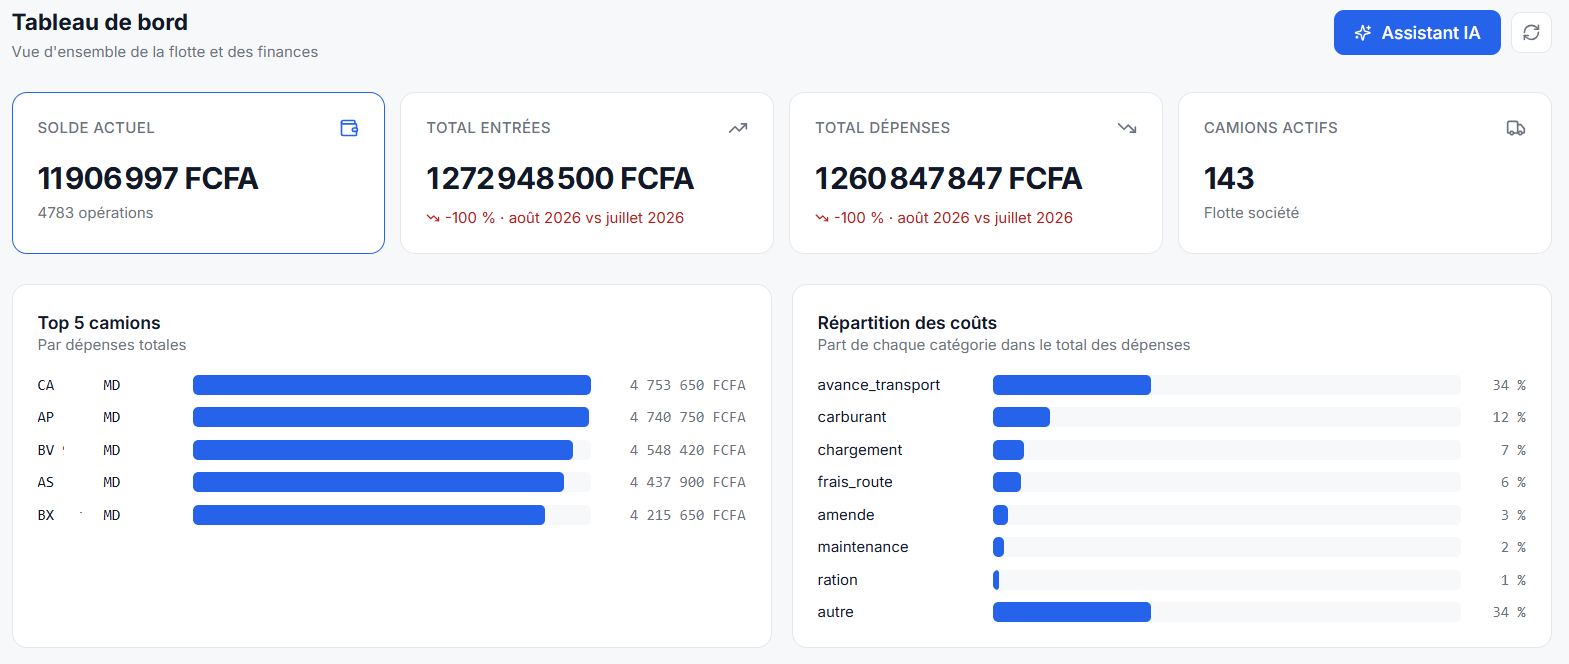
\includegraphics[width=0.85\textwidth]{figures/captures/web_dashboard.png}
    \caption{Tableau de bord : solde, entrées, dépenses, flotte active et répartition des coûts}
    \label{fig:ui_dashboard}
\end{figure}

La vue \textit{Camions} (Figure~\ref{fig:web_flotte}) réalise \texttt{EF-DSH-02} et \texttt{EF-DSH-04} : chaque carte donne l'immatriculation, le pays, la position, le total des dépenses et le nombre d'opérations, et ouvre le profil du camion.

\begin{figure}[H]
    \centering
    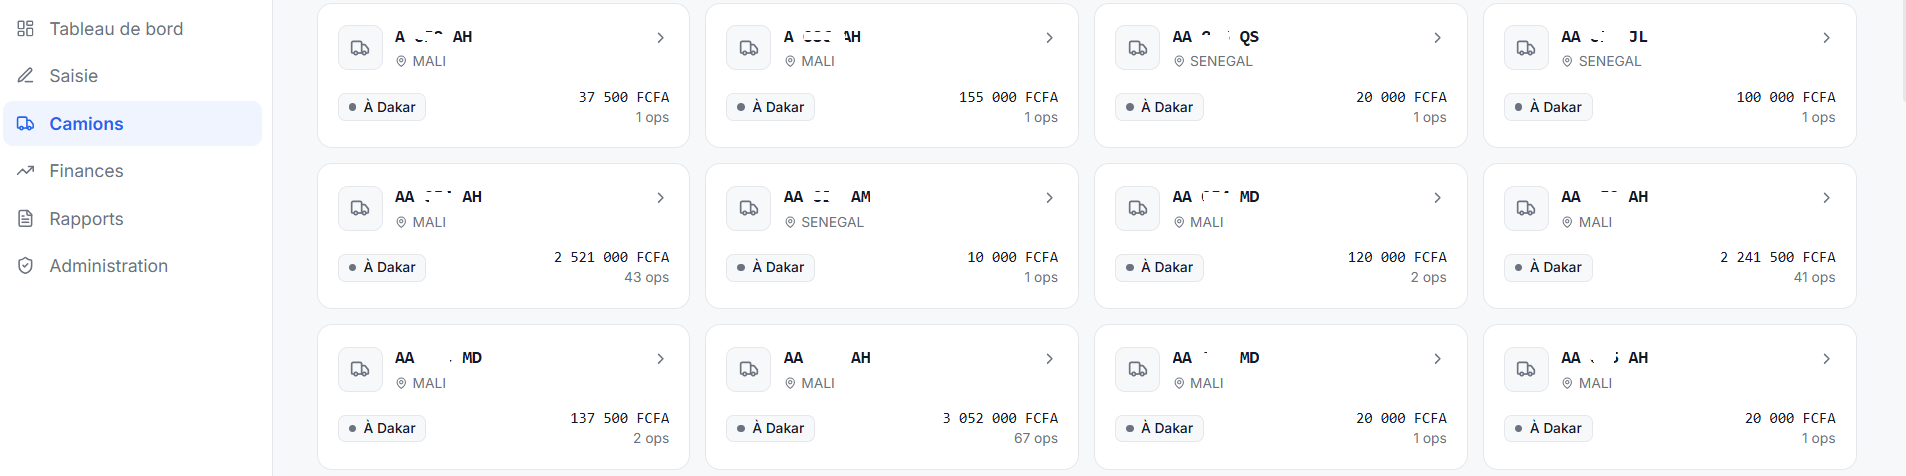
\includegraphics[width=0.85\textwidth]{figures/captures/web_flotte.png}
    \caption{Vue de la flotte par camion}
    \label{fig:web_flotte}
\end{figure}

La saisie directe (Figure~\ref{fig:web_saisie}) remplace le fichier \og RECAP-JOURNALIER \fg{} envoyé par WhatsApp. L'agent choisit le sens de l'opération, puis renseigne le libellé, la date, la catégorie, le montant et, si besoin, le camion et le bon de livraison. L'opération est visible à Bamako dès son enregistrement.

\begin{figure}[H]
    \centering
    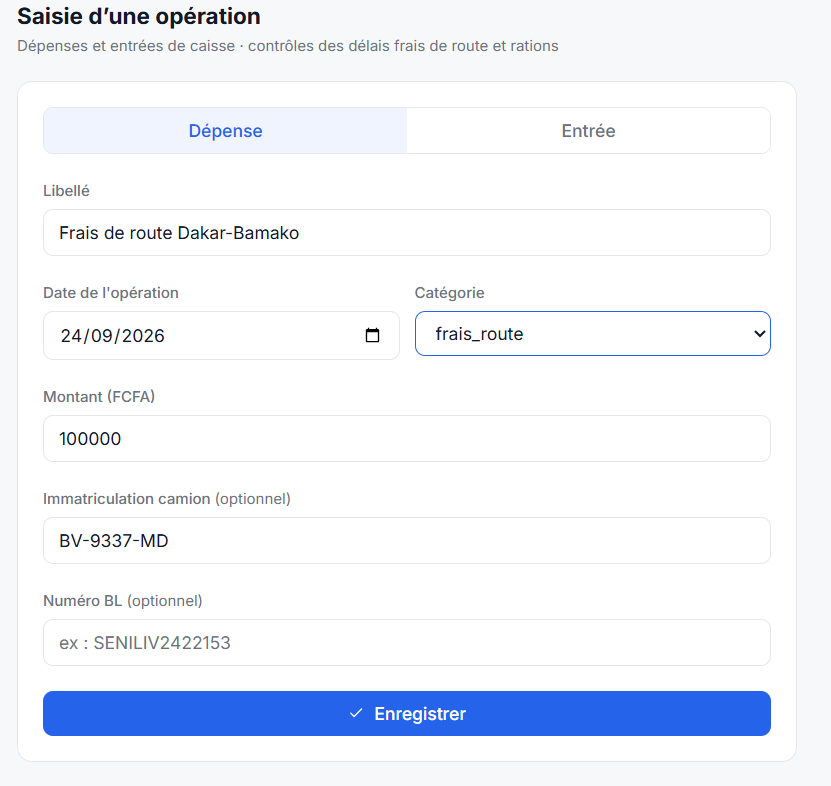
\includegraphics[width=0.5\textwidth]{figures/captures/web_saisie.png}
    \caption{Formulaire de saisie d'une opération de caisse}
    \label{fig:web_saisie}
\end{figure}

\subsection{Authentification et gestion de session}
\label{sec:webapp_jwt}

L'authentification (\texttt{ENF-SEC-01}) repose sur deux jetons. Le jeton d'accès est un JWT signé, valable huit heures ; le serveur refuse de démarrer si sa clé de signature fait moins de 64 caractères. Le jeton de rafraîchissement, valable sept jours, est une chaîne aléatoire dont seule l'empreinte SHA-256 est conservée en base : une fuite de la base ne permet donc de rejouer aucune session. Les mots de passe sont hachés par \texttt{bcrypt} (\texttt{ENF-SEC-02}).

Deux protections dépassent le cahier des charges. Un compte est verrouillé quinze minutes après cinq échecs consécutifs (Figure~\ref{fig:ui_verrouillage}). Et une adresse inconnue déclenche quand même une comparaison \texttt{bcrypt} factice : le temps de réponse ne révèle pas si un compte existe.

\begin{figure}[H]
    \centering
    \begin{minipage}{0.42\textwidth}
        \centering
        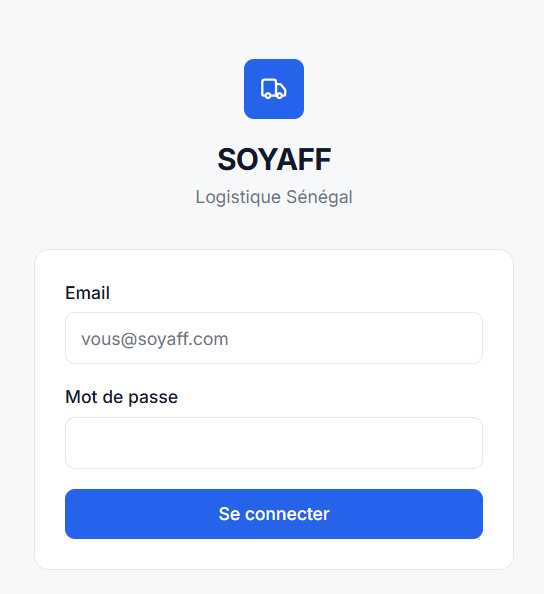
\includegraphics[width=\textwidth]{figures/captures/web_connexion.png}
        \caption{Page de connexion}
        \label{fig:web_connexion}
    \end{minipage}\hfill
    \begin{minipage}{0.48\textwidth}
        \centering
        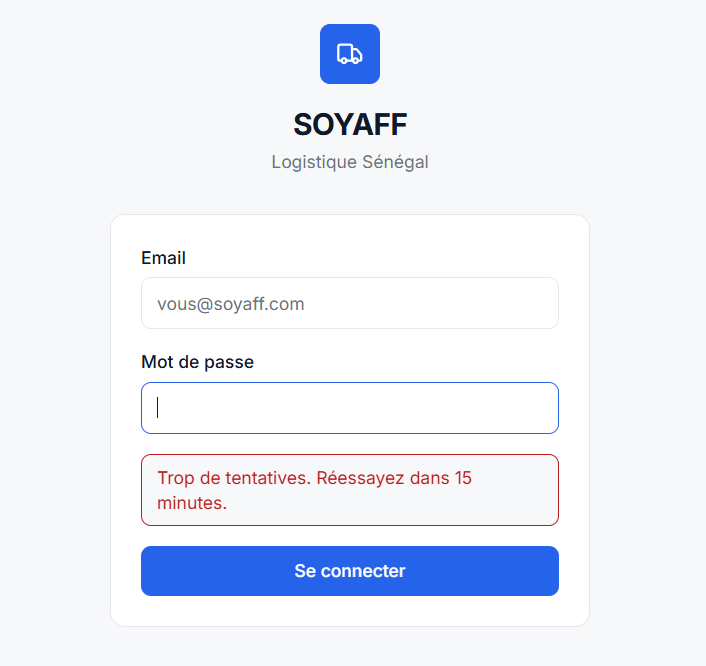
\includegraphics[width=\textwidth]{figures/captures/web_verrouillage.png}
        \caption{Compte verrouillé après cinq échecs}
        \label{fig:ui_verrouillage}
    \end{minipage}
\end{figure}

Deux arbitrages sont assumés. Les jetons sont stockés en \texttt{localStorage}, exposés à un script injecté ; la migration vers des cookies \texttt{httpOnly} est planifiée. Le jeton de rafraîchissement n'est pas renouvelé à chaque usage : il reste valable sept jours, mais la déconnexion le révoque immédiatement.

\subsection{Intégrité des données : le calcul du solde}
\label{sec:webapp_integrity}

Le diagnostic du chapitre~\ref{chap:contexte} relevait des formules de solde qui se cassaient dans les tableurs au fil des copier-coller. Le solde progressif n'est désormais calculé qu'à un seul endroit : la route de saisie \texttt{POST /api/finances/operation}, dans une transaction SQL unique. Elle garantit l'existence du camion et du bon de livraison, relit le dernier solde connu à la date de l'opération, calcule le nouveau solde et l'enregistre avec l'opération. Toute erreur annule l'ensemble : aucune opération ne peut exister sans son solde. Le frontend affiche ce solde sans jamais le recalculer. C'est le même principe que l'idempotence de l'ETL (\S\ref{sec: chargement}) : contraindre la base plutôt que discipliner l'utilisateur.

\subsection{Contrôle des délais de saisie}
\label{sec:webapp_delais}

\texttt{EF-SDR-02} demandait de contrôler l'intervalle entre deux rations d'un même chauffeur. Nous avons étendu ce contrôle aux frais de route, à la suite d'un ordre de travail du 24~septembre~2026. Les règles sont regroupées dans \texttt{utils/delais.js}, couvert par des tests :
\begin{itemize}
    \item \textbf{frais de route} : deux opérations pour un même camion doivent être espacées d'au moins 8~jours, sinon la saisie est bloquée ;
    \item \textbf{rations} : sous 2~jours, la saisie est bloquée ; entre 2 et 5~jours, l'opérateur doit confirmer une alerte.
\end{itemize}
Le chauffeur est rattaché à son camion dans la table \texttt{chauffeurs}. L'écart est mesuré par rapport à l'opération la plus proche, avant \emph{ou} après : une saisie antidatée est contrôlée comme les autres. Le contrôle s'exécute dans l'API, pas seulement dans le formulaire. Seul un administrateur peut lever un blocage ; forçage et confirmation sont inscrits dans \texttt{audit\_logs}. Les Figures~\ref{fig:web_delai_agent} et~\ref{fig:web_delai_admin} montrent la même saisie vue par un agent puis par un administrateur.

\begin{figure}[H]
    \centering
    
\includegraphics[width=0.8\textwidth]{figures/captures/web_delai_agent.png}
    \caption{Frais de route saisi deux fois le même jour, profil agent de Dakar : saisie bloquée}
    \label{fig:web_delai_agent}
\end{figure}

\begin{figure}[H]
    \centering
    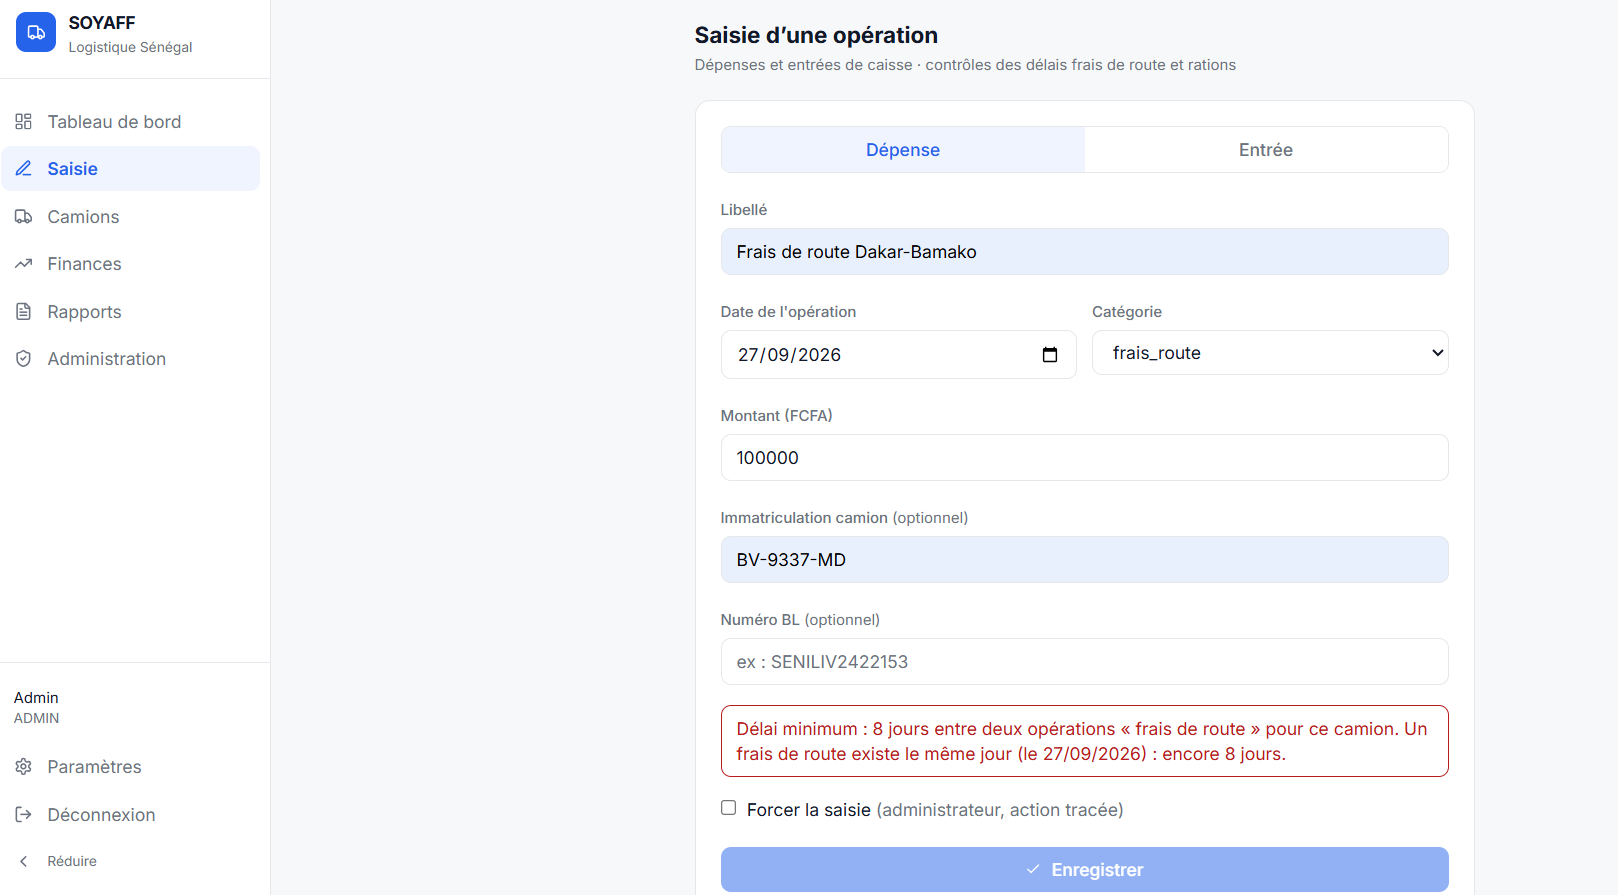
\includegraphics[width=0.7\textwidth]{figures/captures/web_delai_admin.png}
    \caption{Même saisie, profil administrateur : forçage possible et tracé}
    \label{fig:web_delai_admin}
\end{figure}

\subsection{Contrôle d'accès (RBAC) et audit}
\label{sec:webapp_rbac}

Trois rôles (\texttt{DAKAR\_AGENT}, \texttt{BAMAKO\_CHEF}, \texttt{ADMIN}) reprennent les personas de la section~\ref{chap:besoins} (\S\ref{sec:personas}). La liste est contrainte à trois niveaux : l'interface ne propose que ces valeurs, l'API rejette toute autre valeur, et une contrainte \texttt{CHECK} sur la colonne \texttt{users.role} protège la base contre toute écriture qui contournerait l'API (\texttt{ENF-SEC-03}).

Le middleware \texttt{authorize()} vérifie le rôle sur chaque route protégée. En cas de refus, il inscrit lui-même la tentative dans \texttt{audit\_logs} (\texttt{UNAUTHORIZED\_ACCESS}) avant de répondre \texttt{403}. La même table reçoit les actions d'administration réussies : création de compte, changement de rôle, réinitialisation de mot de passe (\texttt{EF-ADM-02}). Elle couvre ainsi les deux volets de \texttt{ENF-SEC-04}, résumés par la Figure~\ref{fig:seq_rbac_audit}. Un administrateur ne peut pas désactiver son propre compte ; désactiver un compte révoque ses sessions ; aucun compte n'est supprimé, pour préserver l'historique d'audit.

\begin{figure}[H]
    \centering
    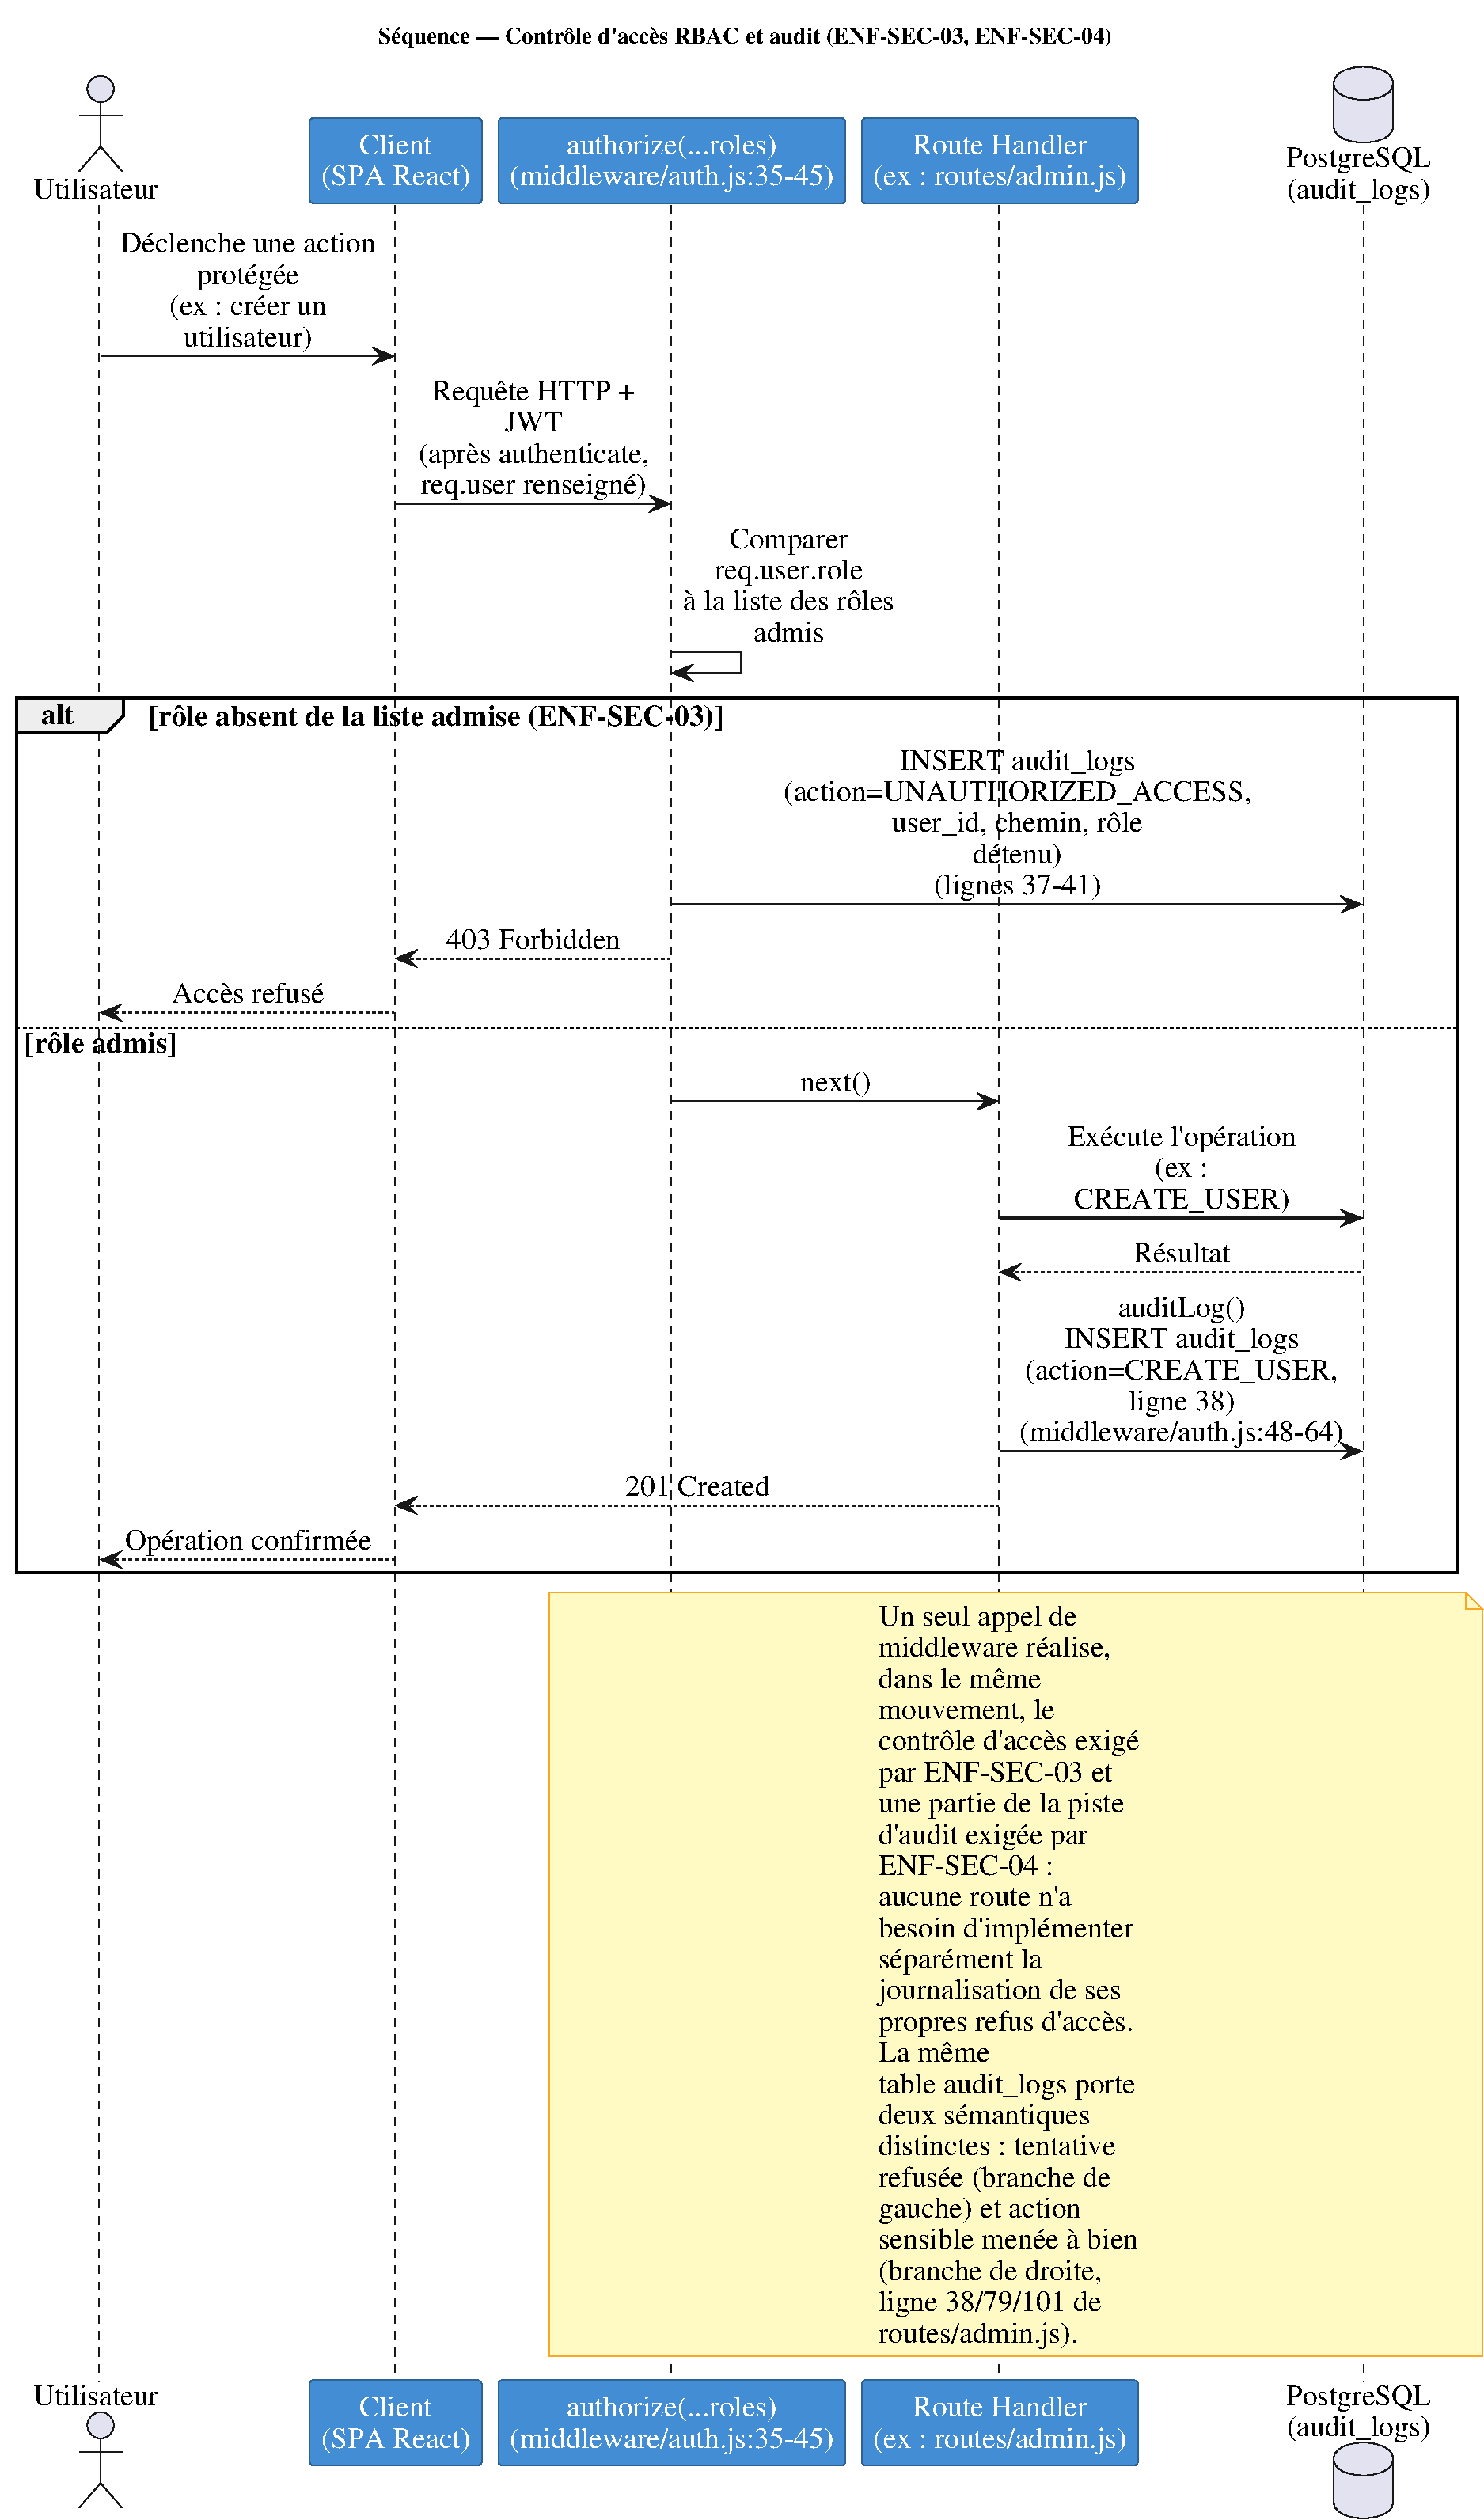
\includegraphics[width=\textwidth,height=0.88\textheight,keepaspectratio]{figures/fig_seq_rbac_audit.pdf}
    \caption{Séquence : contrôle d'accès RBAC et audit}
    \label{fig:seq_rbac_audit}
    \source{Schéma de l'auteur}
\end{figure}

\subsection{Reporting et export}
\label{sec:webapp_reporting}

Les récapitulatifs journalier et mensuel (\texttt{EF-REP-01}, \texttt{EF-REP-02}) et la recherche par période, camion ou catégorie (\texttt{EF-REP-04}) sont déployés. La Figure~\ref{fig:web_rapport} montre le rapport de juillet~2026 : totaux, solde de fin de mois, répartition des dépenses, classement des camions et détail chronologique.

\begin{figure}[H]
    \centering
    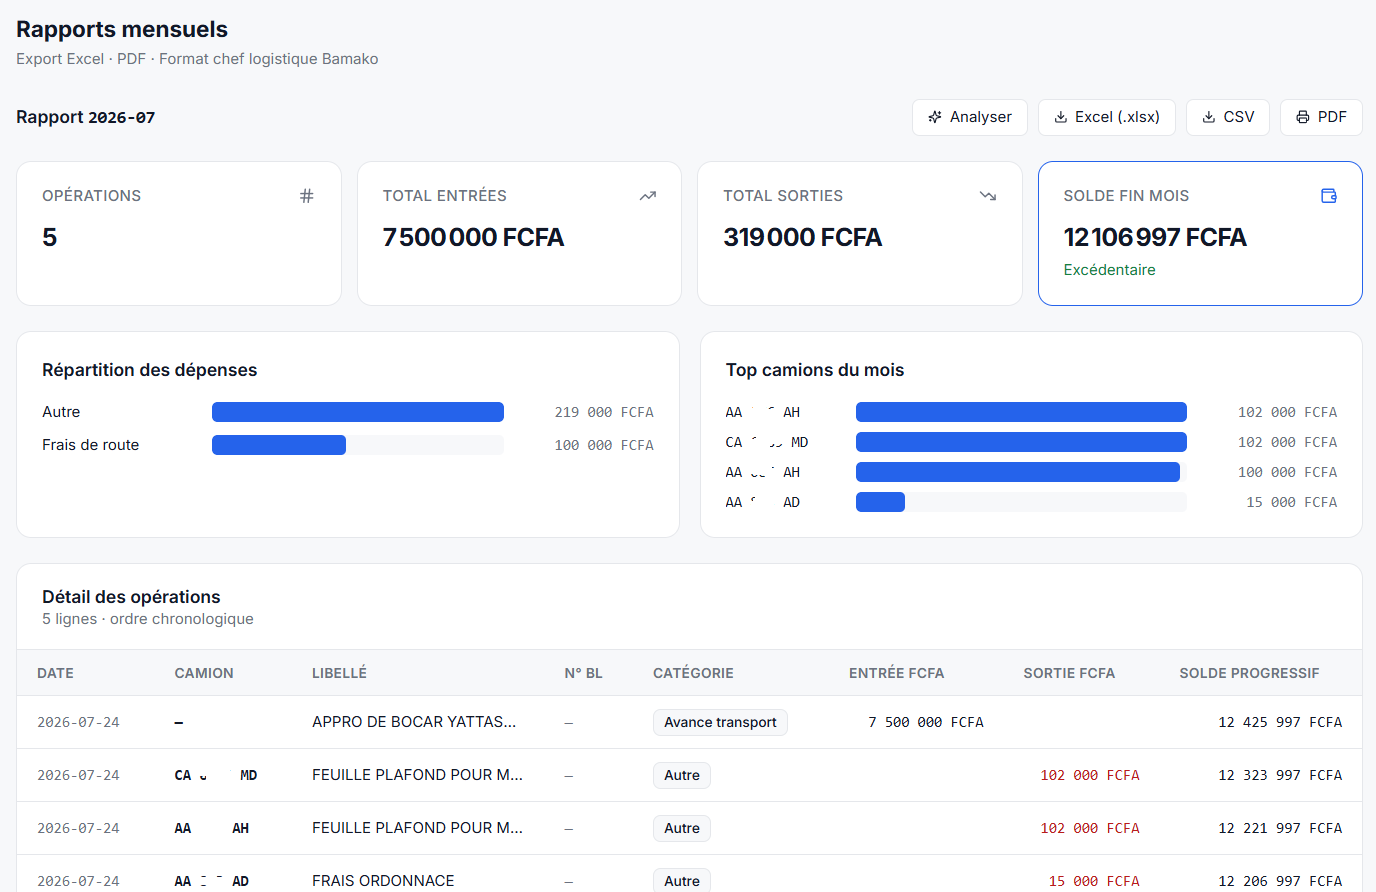
\includegraphics[width=0.75\textwidth]{figures/captures/web_rapport.png}
    \caption{Rapport mensuel consolidé (juillet~2026)}
    \label{fig:web_rapport}
\end{figure}

L'export (\texttt{EF-REP-03}) est partiel. Le CSV respecte l'usage français (encodage UTF-8 avec BOM, séparateur point-virgule) et s'ouvre directement dans Excel. Le fichier Excel est construit par le serveur, avec une feuille de résumé et une feuille de détail (Figure~\ref{fig:web_export}). Le bouton « PDF », en revanche, lance seulement l'impression du navigateur : aucun PDF n'est produit par le serveur. Un vrai export PDF est renvoyé aux perspectives.

\begin{figure}[H]
    \centering
    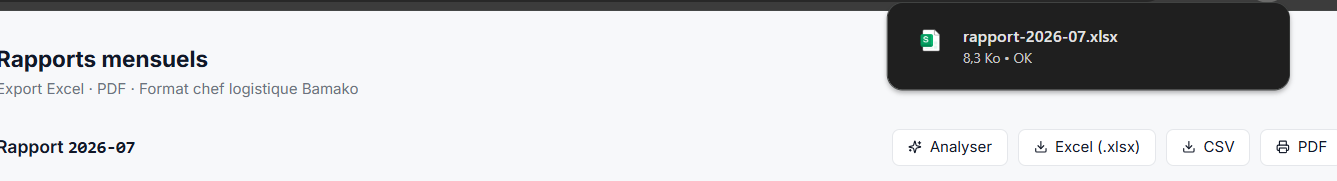
\includegraphics[width=0.8\textwidth]{figures/captures/web_export_xlsx.png}
    \caption{Export Excel du rapport mensuel : fichier \texttt{rapport-2026-07.xlsx} généré par le serveur}
    \label{fig:web_export}
\end{figure}

\subsection{Fonctionnalités cibles non déployées}
\label{sec:webapp_fonctionnalites_cibles_non_deployees}

\textbf{EF-VAL-02 : workflow de validation.} Chaque opération est enregistrée directement et définitivement : il n'existe ni statut (brouillon, validé), ni circuit d'approbation. Le visa manuscrit reste la référence pendant la transition, choix de priorité déjà justifié à la section~\ref{chap:besoins} (\S\ref{sec:synthese_tracabilite}) et représenté par le diagramme d'activité cible (Figure~\ref{fig:activite_validation_cible}).

\textbf{ENF-DISP-01 : mode hors-ligne.} Aucun mécanisme de saisie hors connexion n'existe : c'est une cible non entamée.

Ces deux manques ne remettent en cause ni la fin de la double saisie ni la visibilité en temps réel, déjà obtenues. Leur priorisation est discutée à la section~\ref{chap:discussion}.

\subsection{Synthèse et transition}
\label{sec:webapp_synthese_transition}

L'application réalise le cœur du cahier des charges : saisie unique et contrôlée, solde calculé par la base, accès cloisonné par rôle avec piste d'audit, rapports et exports. Elle reste une exploitation structurée, par formulaires et filtres. L'interrogation des données en langage naturel fait l'objet de la section suivante.
